\section{Principal Component Analysis}\label{sec:PCA}
%
%
\subsection{Principal Component Analysis, the classical statistical tool}
The Principal Component Analysis (PCA) \cite{fisher1938statistical} is a statistical technique for data dimensionality reduction. It looks for the so-called {\em Principal Components} (PCs for short), which are vectors that form an orthonormal basis for $\mathbb{R}^\traceLength$ (\textit{i.e.} these vectors have norm equal to 1 and are orthogonal to each other). Such PCs are computed, via singular value decomposition, as the eigenvectors of the empirical covariance matrix of data: given a set of data $(\sss[]{i})_{i=1,\dots,\numTraces[]},$ the empirical covariance matrix is given by:
\begin{equation}\label{eq:covmat}
\covmat = \frac{1}{\numTraces[]} \sum_{i=1}^{\numTraces[]}(\sss[]{i} - \mmmX)(\sss[]{i} - \mmmX)^\intercal \mbox{ ,}
\end{equation}
 where $\mmmX$ is the empirical mean of data. Let us denote by $r$ the rank of $S$ and by $\AAlpha_1, \dots, \AAlpha_r$ and $\lambda_1, \dots, \lambda_r$ its eigenvectors and the corresponding eigenvalues, respectively. We assume that the $\AAlpha_i$ are listed in the decreasing order of the values $\lambda_i$. It can be shown that $\lambda_i$, for each $i$, equals the empirical variance of the data projected onto the corresponding PC $\AAlpha_i$. Since the data variability is associated to the amount of information, transforming data over the basis provided by the PCs allows a dimensionality reduction that reinforces such information: that is projecting the data onto the  $\newTraceLength$-dimensional subspace of $\mathbb{R}^\traceLength$ spanned by the $\newTraceLength$ leading PCs, or equivalently construct the matrix $A$ of $\eqref{eq:linearExtractor}$ storing as rows the $\newTraceLength$ leading PCs, transposed.\\

\subsection{Principal Component Analysis, the {\em Class-Oriented Version}}\label{sec:PCA_classes}
In SCA context, the useful information part contained in data is the one that allows to discriminate observations linked to different intermediate computations. Let us denote by $\sensRandVar = \targetFunction(\randPlaintext,\randKey)$ the target intermediate variable, that depends on both a secret variable $\randKey$ and on a public one $\randPlaintext$, and that takes values $\sensVar \in \sensVarSet$. An SCA efficiency clearly depends on the ability of the involved extractor to amplify the distinguishability between traces associated to different $\sensVar$.\\

During the profiling phase the attacker is assumed to know the value $\sensVar$ of the sensitive variable handled during each acquisition. She can therefore assign the {\em class} $\sensVar$ to each profiling trace  (in analogy with the pattern recognition terminology), obtaining the labelled profiling set $(\sss{i})_{i=1,\dots,\numTraces}$, where $\numTraces$ is the number of traces belonging to the class $\sensVar$. This knowledge is very useful to construct a good class-distinguishing extractor, but the classical PCA does not exploit it. For this reason in SCA literature \cite{TAprincipal,choudaryefficient,choudary2014efficient,disassembler,Standaert2008}  a {\em class-oriented} version of PCA is often used instead of the classical one. Let $\mmmXclass$ be the empirical mean of traces belonging to the same class $\sensVar$. The class-oriented version of the PCA  consists in applying the PCA dimension reduction to the set $(\mmmXclass)_{\sensVar \in \sensVarSet}$, instead of applying it directly to the traces $\sss{i}$. This implies that the empirical covariance matrix will be computed using only the $\lvert \sensVarSet \rvert$ average traces. Equivalently, in case of \textit{balanced} acquisitions ($\numTraces$ constant for each class $\sensVar$), it amounts to replace the covariance matrix $\covmat$ of data in \eqref{eq:covmat}  by the so-called {\em between-class} or inter-class {\em scatter matrix}, given by:
\begin{equation}\label{eq:SB}
\SB = \sum_{\sensVar\in\sensVarSet}\numTraces(\mmmXclass-\mmmX)(\mmmXclass-\mmmX)^\intercal \mbox{ .}
\end{equation}
Remark that $\SB$ coincides, up to a multiplicative factor, to the covariance matrix obtained using the class-averaged traces.\\

Performing PCA (or LDA as we will see in next section) always requires to compute the eigenvectors of some symmetric matrix $\covmat$, essentially obtained by multiplying a matrix $\measuresMatrix$ with its transposed (e.g. for class-oriented PCA we have $\measuresMatrix = [\sqrt{\numTraces[\sensVar_1]}(\mmmXclass[\sensVar_1]-\mmmX),\sqrt{\numTraces[\sensVar_2]}(\mmmXclass[\sensVar_2]-\mmmX), \dots ]$). Let $\measuresMatrix$ have dimension $\traceLength\times\numTraces[]$, and suppose $\numTraces[]\ll \traceLength$ (which occurs for example in class-oriented PCA , since $\numTraces[]=\lvert \sensRandVar \rvert$). Then, the matrix $\covmat=\measuresMatrix\measuresMatrix^\intercal$ has rank at most $\numTraces[]$. Moreover, rows of $\measuresMatrix$ are often linearly dependent (as in our example since they are forced to have zero mean), so the rank of $\covmat$ is actually strictly less than $\numTraces[]$, giving us at most $\numTraces[]-1$ eigenvectors.\\

A practical problem when $\traceLength$ is large, which happens e.g. when attacking RSA, is represented by the computation and the storage of the $\traceLength\times\traceLength$ matrix $\covmat$. Archambeau et al. \cite{TAprincipal} proposed a method that circumvents this issue, allowing computing the eigenvectors of low-rank big-dimensional symmetric matrices without computing and storing such matrices. In next section we will observe in which cases such a method can be applied to LDA and for which LDA variants.

%\subsection{Computational Trick to Avoid the Computation of Big Covariance Matrices}
%Performing PCA (or LDA, as we will see in next section), always requires to compute the eigenvectors of some symmetric matrix $\covmat$, essentially obtained by a matrix $\measuresMatrix$ with its transposed(e.g. for class-oriented PCA we have $\measuresMatrix = [\sqrt{\numTraces[\sensVar_1]}(\mmmXclass[\sensVar_1]-\mmmX),\sqrt{\numTraces[\sensVar_2]}(\mmmXclass[\sensVar_2]-\mmmX), \dots ]$). Let $\measuresMatrix$ have dimension $\traceLength\times\numTraces[]$, and suppose $\numTraces[]\ll \traceLength$ (which occurs for example in class-oriented PCA , since $\numTraces[]=\lvert \sensRandVar \rvert$). Then, the matrix $\covmat=\measuresMatrix\measuresMatrix^\intercal$ is far from being a full-rank matrix and we can obtain at most $\numTraces[]$ eigenvectors. Moreover, rows of $\measuresMatrix$ are often linearly dependent (as in our example since they are forced to have zero mean), so the rank of $\covmat$ is actually strictly less than $\numTraces[]$, giving us at most $\numTraces[]-1$ eigenvectors.\\
%A practical problem in case of high-dimensional data, i.e. when $\traceLength$ is big, which happens e.g. when attacking RSA, is represented by the computation and the storage of the $\traceLength\times\traceLength$ matrix $\covmat$. This problem can be circumvented by exploiting the following lemma coming from linear algebra:
%\begin{lemma}
%For any $\traceLength\times\numTraces[]$ matrix $\measuresMatrix$, mapping $\xxx\mapsto \measuresMatrix \xxx$ is a one-to-one mapping that maps eigenvectors of  $\measuresMatrix^\intercal\measuresMatrix$ ($\numTraces[]\times\numTraces[]$)    onto those of   $\measuresMatrix\measuresMatrix^\intercal$ ($\traceLength\times\traceLength$).
%\end{lemma}
%%
%This lemma allows to compute and store the $\numTraces[]\times\numTraces[]$ matrix $\tilde{\covmat} = \frac{1}{\numTraces[]}\measuresMatrix^\intercal\measuresMatrix$, compute its $\numTraces[]\times 1$ eigenvectors $\BBeta_i$ and eigenvalues $\lambda_i$, convert them into eigenvectors of $\covmat$: $\AAlpha_i = \measuresMatrix\BBeta_i$. It is not guaranteed that eigenvectors $\AAlpha$ obtained in this way have norm equal to 1. This is why a normalization step should follow if we aim to obtain an orthonormal set of eigenvectors.


\subsection{The Open Question: Choosing the Components to Keep?}\label{sec:ELV}
The introduction of the PCA method in SCA context (either in its classical or class-oriented version)  has raised some important questions: \textit{how many} principal components and \textit{which ones} are sufficient/necessary to reduce the trace size (and thus the attack processing complexity) without losing important discriminative information?\\

Until now, an answer to the questions above has been given in \cite{choudary2014efficient}, linked to the concept of {\em explained variance} (or {\em explained global variance}, EGV for short) of a PC $\AAlpha_i$:
\begin{equation}\label{eq:EGV}
\mathrm{EGV}(\AAlpha_i) =  \frac{\lambda_i}{\sum_{k=1}^r\lambda_k} \mbox{ ,}
\end{equation}
where $r$ is the rank of the covariance matrix $\covmat$, and $\lambda_j$ is the eigenvalue associated to the $j$-th PC $\AAlpha_j$. $\mathrm{EGV}(\AAlpha_i)$ is the variance of the data projected over the $i$-th PC (which equals $\lambda_i$) divided by the total variance of the original data (given by the trace of the covariance matrix $\covmat$). By definition of EGV, the sum of all the EGV values is equal to $1$; that is why this quantity is often multiplied by $100$ and expressed as percentage.
Exploiting the EGV to choose among the PCs consists in fixing a wished {\em Cumulative Explained Variance} $\beta$ and in keeping $\newTraceLength$ different PCs, where $\newTraceLength$ is the minimum integer such that
\begin{equation}
\mbox{EGV}(\AAlpha_1) +\mbox{EGV}(\AAlpha_2) + \dots +\mbox{EGV}(\AAlpha_\newTraceLength) \geq \beta \mbox{ .}
\end{equation}
However, if the adversary has a constraint for the reduced dimension $\newTraceLength$, the EGV notion simply suggests to keep the first $\newTraceLength$ components, taking for granted that the optimal way to chose PCs is in their natural order. This assumption is not always confirmed in SCA context: in some works, researchers have already remarked that the first components sometimes contain more noise than information \cite{Batina2012,specht} and it is worth discarding them. For the sake of providing a first example of this behaviour on publicly accessible traces, we applied a class-oriented PCA on 3000 traces from the DPA contest v4 \cite{DPAcontest}; we focused over a small 1000-dimensional window in which, in complete knowledge about masks and other countermeasures, information about the first Sbox processing leaks (during the first round). In Fig.~\ref{fig:DPAcontest} the first and the sixth PCs are plotted. It may be noticed that the first component indicates that one can attend a high variance by exploiting the regularity of the traces, given by the clock signal, while the sixth one has high coefficients localised in a small time interval, very likely to signalize the instants in which the target sensitive variable leaks.

\begin{figure}
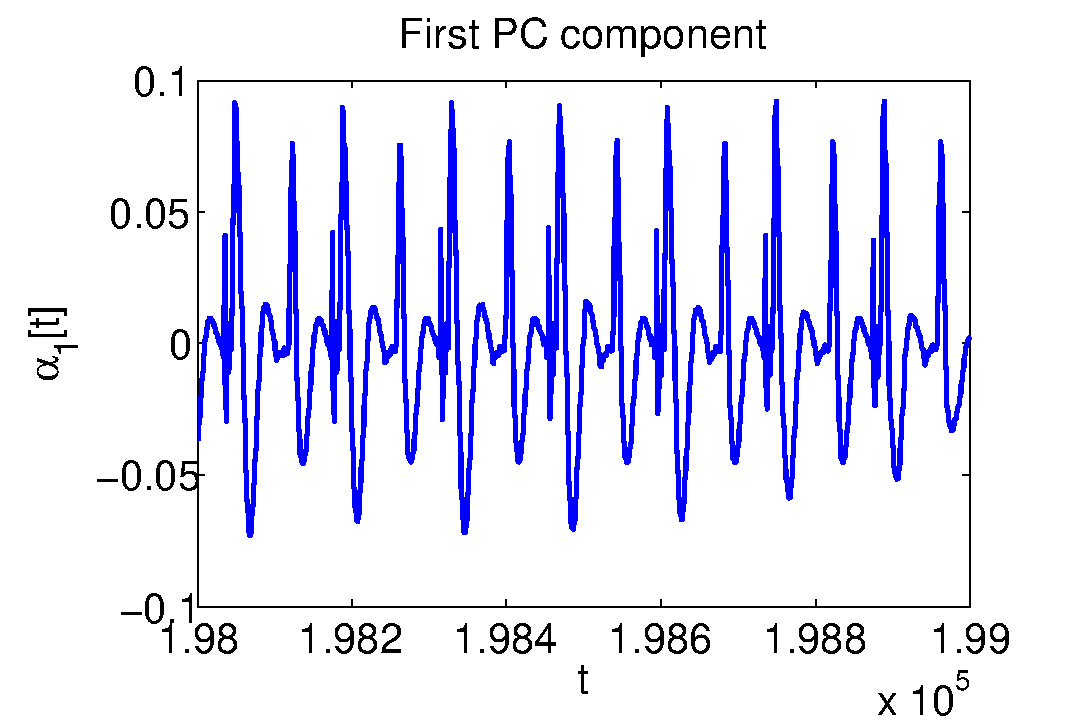
\includegraphics[width=.45\textwidth]{figures/DPAcontestPC1.pdf} 
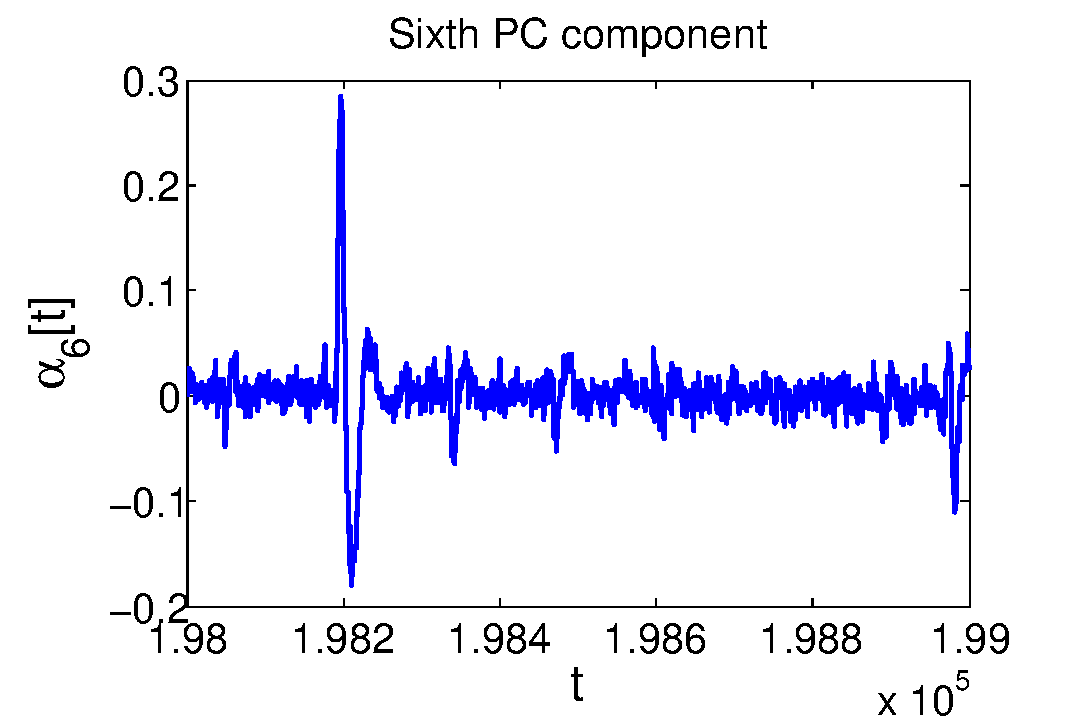
\includegraphics[width=.45\textwidth]{figures/DPAcontestPC6.pdf} 
\caption{First and sixth PCs in DPA contest v4 trace set}\label{fig:DPAcontest}
\end{figure}
To the best of our knowledge, a single method adapted to SCA context has been proposed until now to automatically chose PCs \cite{SCAclassProbl} while dealing with the issue raised in Fig.~\ref{fig:DPAcontest}. It is based on the following assumption:
\begin{assumption}\label{assum:local}
The leaking side-channel information is localised in few points of the acquired trace.
\end{assumption}
In the rest of the paper, we conduct our own analyses under Assumption \ref{assum:local} that we think to be reasonable in SCA contexts where the goal of the security developers is to minimize the number of leaking points.
Under this assumption, the authors of \cite{SCAclassProbl} propose a measure to evaluate the eigenvectors {\em localization}. It is called {\em Inverse Participation Ratio} (IPR) and is defined as follows:
\begin{equation}
\mathrm{IPR}(\AAlpha_i) = \sum_{j=1}^\traceLength \AAlpha_i[j]^4 \mbox{ .}
\end{equation}
The authors of \cite{SCAclassProbl} suggest to collect the PCs in decreasing order with respect to the IPR score.\\

The selection methods provided by the evaluation of the EGV and of the IPR are somehow complementary: the former is based only on the eigenvalues associated to the PCs and does not consider the form of the PCs themselves; the latter completely discards the information given by the eigenvalues of the PCs, considering only the distribution of their coefficients. One of the contributions of the present paper is to propose a new selection method, that builds a bridge between the EGV and the IPR approaches. As we will argue, our method, based on the so-called {\em Explained Local Variance}, does not only lead to the construction of a new selection criterion, but also permits  to modify the PCs, choosing individually the coefficients to keep and those to discard. 

\subsection{The Explained Local Variance Selection Method} 
The method we develop in this section is based on a compromise between the variance provided by each PC (more precisely its EGV) and the number of time samples necessary to achieve a consistent part of such a variance. To this purpose we  introduce the concept of {\em Explained Local Variance} (ELV).
\begin{figure}
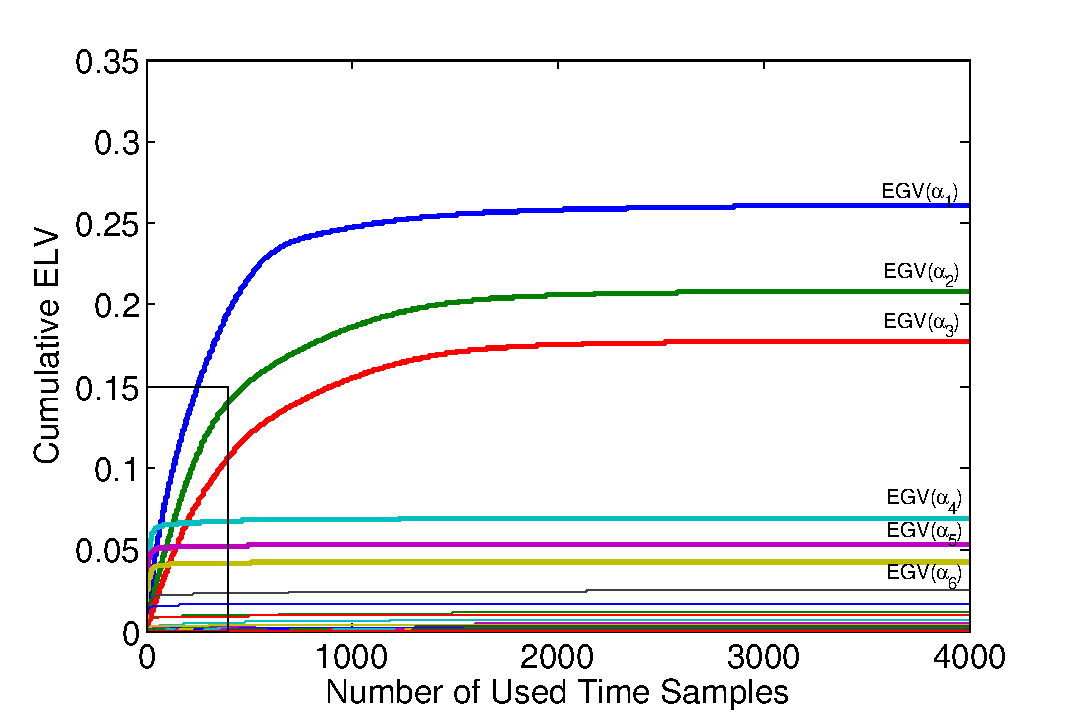
\includegraphics[width=0.5\textwidth]{figures/cumulativeELVallRectangle.pdf} 
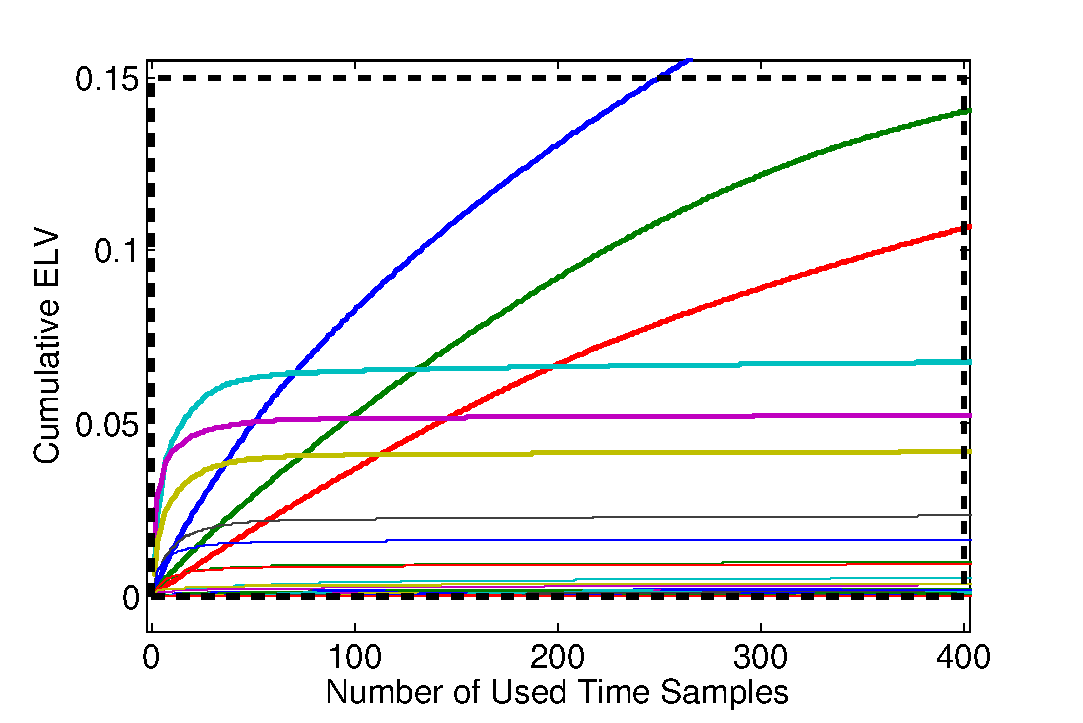
\includegraphics[width=0.5\textwidth]{figures/cumulativeELVzoomedRectangle.pdf} 
\caption{Cumulative ELV trend of principal components. On the right a zoom of the plot on the left. Data acquisition described in Sec.~(\ref{sec:fourCriteria}).}\label{fig:ELVcumulative}
\end{figure}

Let us start by giving some intuition behind our new concept. Thinking to the observations ${\sss[]{}}^\intercal$, or to the class-averages ${\mmmX}^\intercal$ in class-oriented PCA case, as realizations of a random variable $\XXX^\intercal$, we have that $\lambda_i$ is an estimator for the variance of the random variable $\XXX^\intercal\cdot\AAlpha_i$. Developing, we obtain
\begin{align}\label{eq:ELV}
\lambda_i =& \hat{\mathrm{var}}(\sum_{j=1}^D \XXX^\intercal[j]\AAlpha_i[j]) = \sum_{j=1}^D\sum_{k=1}^D \hat{\mathrm{cov}}(\XXX^\intercal[j]\AAlpha_i[j], \XXX^\intercal[k]\AAlpha_i[k])=\\
=& \sum_{j=1}^D \AAlpha_i[j]\sum_{k=1}^D\AAlpha_i[k]\hat{\mathrm{cov}}(\XXX^\intercal[j], \XXX^\intercal[k])= \sum_{j=1}^D \AAlpha_i[j] (\covmat_{j}^\intercal \cdot \AAlpha_i)=  \\
=& \sum_{j=1}^D \AAlpha_i[j] \lambda_i\AAlpha_i[j]= \sum_{j=1}^D  \lambda_i \AAlpha_i[j]^2 \label{eq:toJustify}
\end{align}
where $\covmat_{j}^\intercal$ denotes the $j$-th row of $\covmat$ and \eqref{eq:toJustify} is justified by the fact that $\AAlpha_i$ is an eigenvector of $\covmat$, with $\lambda_i$ its corresponding eigenvalue. The result of this computation is quite obvious, since $\parallel \AAlpha_i\parallel=1$, but it evidences the contribution of each time sample in the information held by the PC. This makes us introduce the following definition:
\begin{definition}


The {\em Explained Local Variance} of a PC $\AAlpha_i$ in a sample $j$, is defined by
\begin{equation}
\mathrm{ELV}(\AAlpha_i,j) = \frac{\lambda_i \AAlpha_i[j]^2}{\sum_{k=1}^r\lambda_k} = \mathrm{EGV}(\AAlpha_i) \AAlpha_i[j]^2  \mbox{ .}
\end{equation}
\end{definition}
\begin{figure}
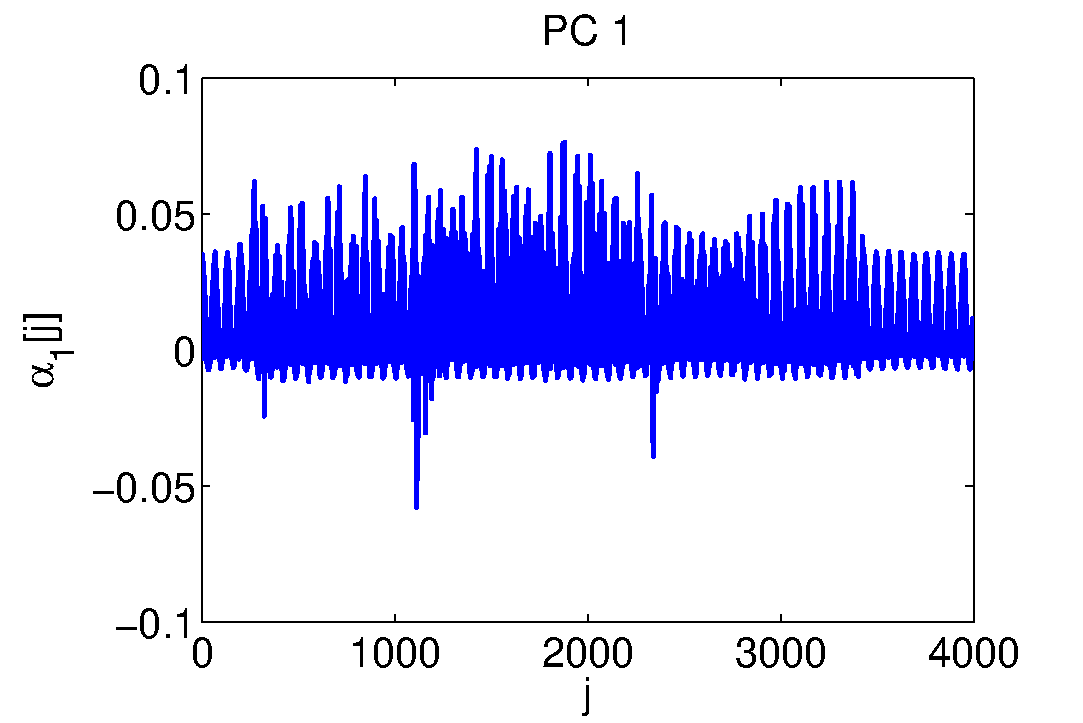
\includegraphics[width=0.31\textwidth]{figures/PC1.pdf} 
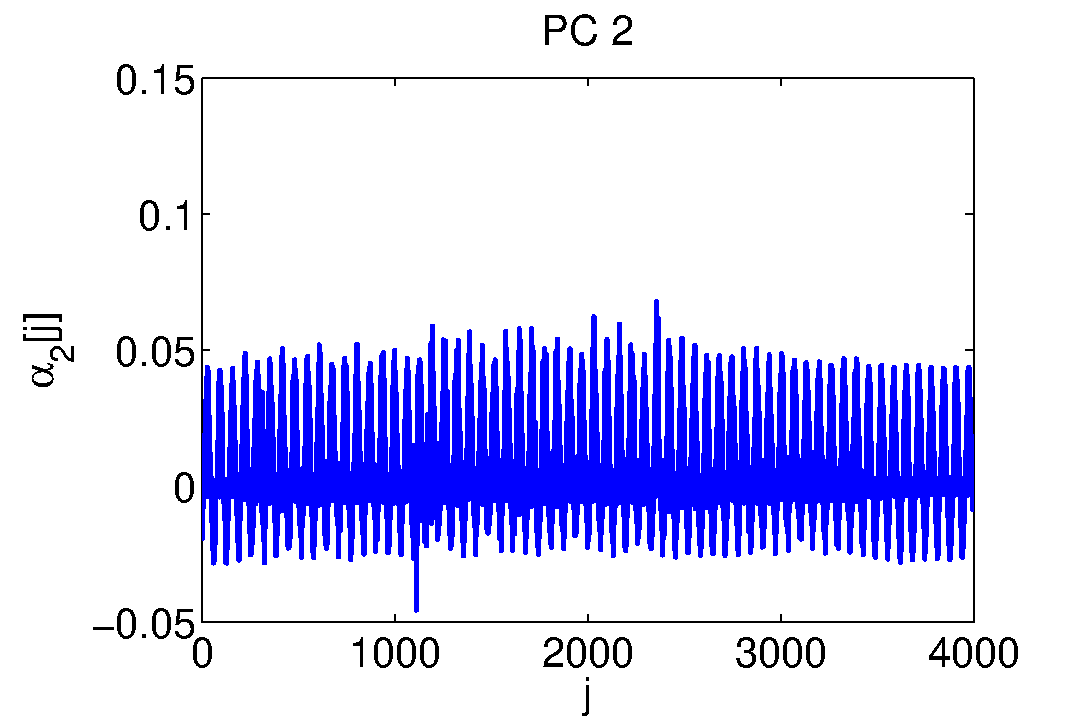
\includegraphics[width=0.31\textwidth]{figures/PC2.pdf} 
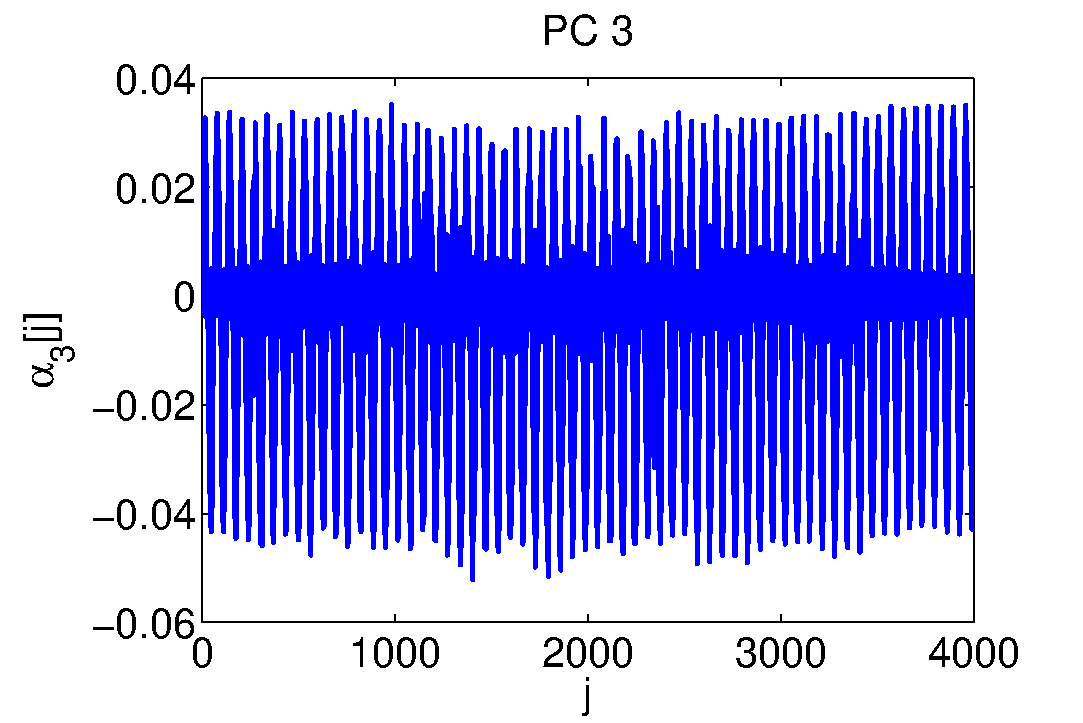
\includegraphics[width=0.31\textwidth]{figures/PC3.pdf} \\
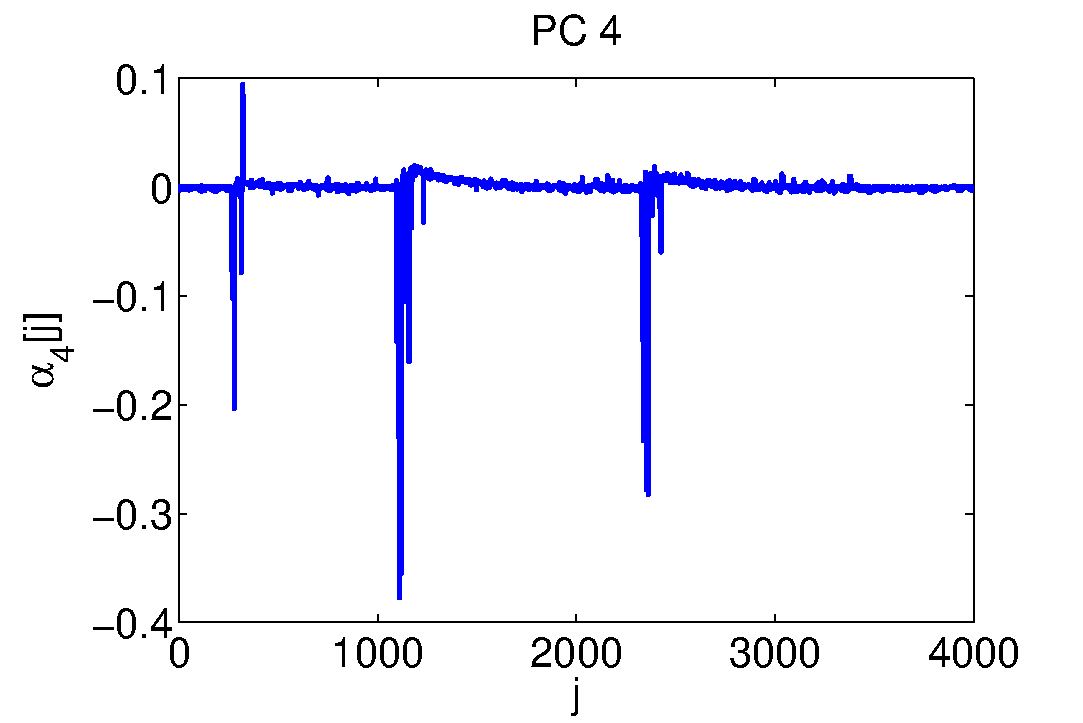
\includegraphics[width=0.31\textwidth]{figures/PC4.pdf} 
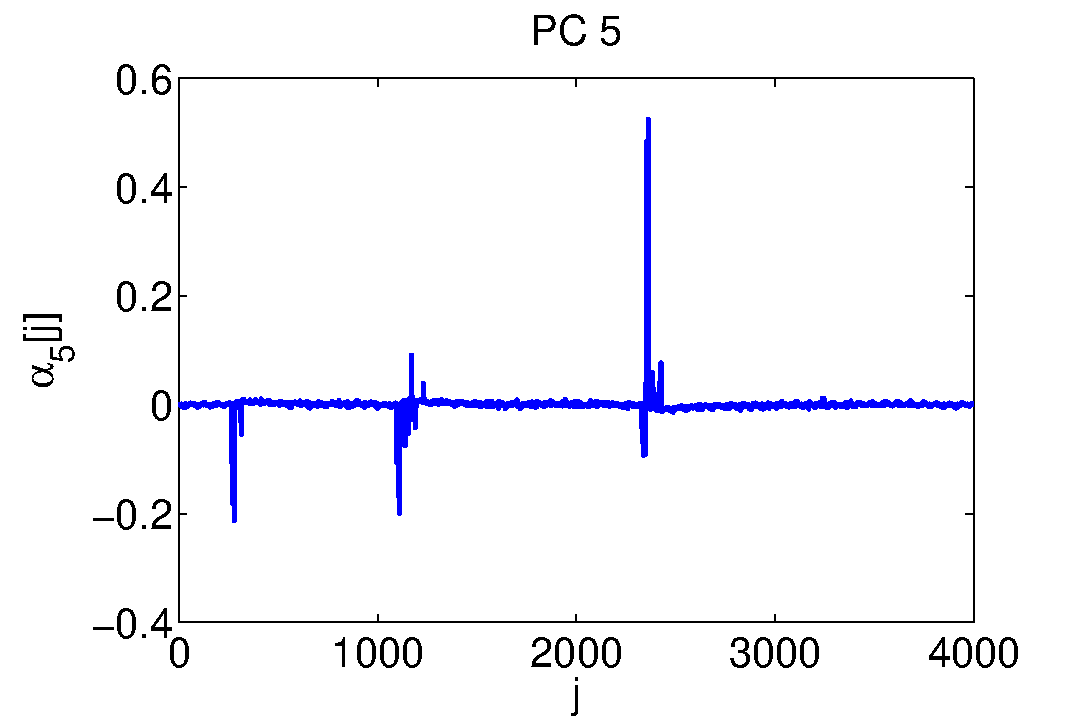
\includegraphics[width=0.31\textwidth]{figures/PC5.pdf} 
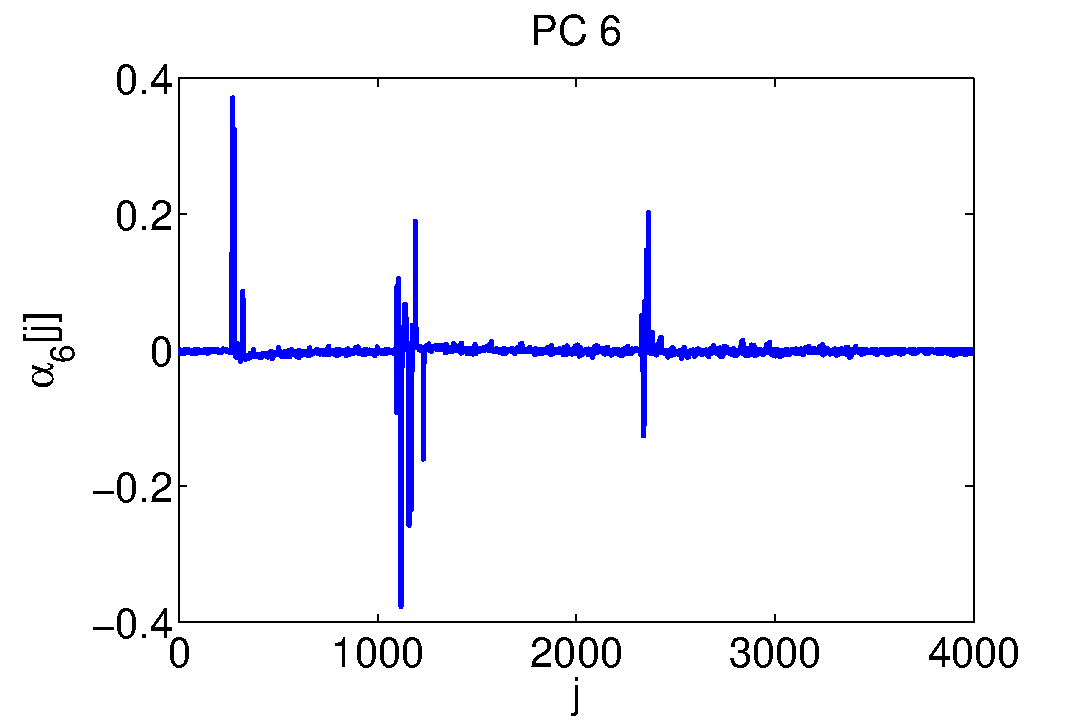
\includegraphics[width=0.31\textwidth]{figures/PC6.pdf} 
\caption{The first six PCs. Acquisition campaign on an 8-bit AVR Atmega328P (see Sec.~\ref{sec:experiments}).}\label{fig:6components}
\end{figure}
It may be observed that the sum over all the trace samples ELVs of a PC equals the EGV of the considered PC. If we operate such a sum for each PC in a cumulative way and in decreasing order over the coefficients starting from the one that holds the maximal ELV, we obtain a complete description of the trend followed by each component to achieve its EGV. As we can see in Fig.~\ref{fig:ELVcumulative}, where such cumulative ELVs are represented, the first 3 components are much slower in achieving their final EGV, while the $4^\text{th}$, the $5^\text{th}$ and the $6^\text{th}$ achieve a large part of their final EGVs very quickly ({\em i.e.} by adding the ELV contributions of much less time samples). This implies that the EGV of the $4^\text{th}$, the $5^\text{th}$ and the $6^\text{th}$ only essentially depends on a very few time samples. This observation, combined with Assumption \ref{assum:local}, suggests that they are more suitable for SCA than the three first ones. To validate this statement, it suffices to look at the form of such components (Fig.~\ref{fig:6components}): the leading ones are very influenced by the clock, while the latest ones are well localised over the leaking points.\\

Operating a selection of components {\em via} ELV, in analogy with the EGV, requires to fix the reduced space dimension $\newTraceLength$, or a threshold $\beta$ for the cumulative ELV. In the first case, the maximal ELVs of each PC are compared, and the $\newTraceLength$ components achieving the highest values of such ELVs are chosen. In the second case, all couples (PC, time sample) are sorted in decreasing order with respect to their ELV, and summed until the threshold $\beta$ is achieved. Then only PCs contributing in this sum are selected. \\

We remark that the ELV is a score associated not only to the whole components, but to each of their coefficients. This interesting property can be exploited to further remove, within a selected PC, the non-significant points, {\em i.e.} those with a low ELV. In practice this is done by setting these points to zero. That is a natural way to exploit the ELV score in order to operate a kind of {\em denoising} for the reduced data, making them only depend  on the significant time samples. In Sec.~\ref{sec:experiments} (scenario 4) we test the performances of an attack varying the number of time samples involved in the computation of the reduced data, and showing that such a denoising processing might impact significantly. 
 


%Actually, the ELV selection method, in analogy with the EGV one, consists in fixing a threshold value $\beta$ for the wished {\em Cumulative Explained Local Variance} and in constructing the set 
%\begin{equation}
%S = \{(i_1, t_1), \dots , (i_{\newTraceLength},t_{\newTraceLength})\} 
%\end{equation}
%where $\newTraceLength$ is the minimal integer such that
%\begin{equation}
%\mathrm{ELV}(i_1,t_1)+\dots +  \mathrm{ELV}(i_{\newTraceLength},t_{\newTraceLength})\geq \beta \mbox{ .}
%\end{equation}
%The rule to choose PCs to keep is then
%\begin{equation}
%\mbox{Keep } \AAlpha_i \Leftrightarrow \exists t \mbox{ such that } (i,t)\in S \mbox{; }
%\end{equation}
%moreover, we propose to only consider, among time samples of each chosen PC, those that hold a significant ELV. For this reason we suggest to consider new PCs $\tilde{\AAlpha}_i$, that we believe incorporate less noise, constructed as follows:
%
%\begin{equation}
%\tilde{\AAlpha}_i[t] = \begin{cases}
%\AAlpha_i[j] \mbox{ if } (i,t)\in S\\
%0 \mbox{ otherwise.}
%\end{cases}
%\end{equation}



%Moreover we define the {\em ELV vector} of a PC $\AAlpha_k$ as the vector $\vectorContribution = (\mathrm{ELV}(k,i))_{i=1..\traceLength}$.
%\end{definition}
%
%
%\subsubsection{{\em Cumulative Explained Local Variance} selection method}
%In this section we present how to select the most informative PCs and how to modify them in order to meaningfully obtain interesting PVs for side channels context.\\
%
%Let $r$ be the rank of the covariance matrix $\covmat$, i.e. the total number of PCs, $\AAlpha_1, \dots, \AAlpha_r$.\\
%Let $\coupleSet = \{1,\dots, r\}\times \{1,\dots,\traceLength\}$ and let us introduce a succession of index couples as
%
%\begin{equation}
%\begin{cases}
%(k_1, i_1) = \mathrm{argmax_{(k,i)\in \coupleSet}}\mathrm{ELV}(k,i)\\
%(k_j, i_j) = \mathrm{argmax_{(k,i)\in \coupleSet\smallsetminus \{(k_1,i_1),\dots,(k_{j-1}, i_{i-1})\}}}\mathrm{ELV}(k,i)\mbox{ .}
%\end{cases}
%\end{equation}
%
%Now fix 
%
%\begin{remark}
%Let $A$ be the matrix that contains the chosen $\tilde{\AAlpha}_k$ vectors as columns. The total variance $\sum diag(A^\intercal\covmat A)$ will not attend the  $\beta$-th part of the initial variables variance, as it would be if eigenvectors $\AAlpha_k$ would have been kept unchanged, but will be lower than it. This is exactly because  vectors $\tilde{\AAlpha}_k$ are no more eigenvectors of $\covmat$. 
%\end{remark}
%
%
%\paragraph{A practical problem that might occur: linear dependent projected data}
%Since the proposed method suggests changing the PCs into new projecting vectors $\tilde{\AAlpha}_k$, the property of decorrelating principal variables is lost. On the contrary it might happen, especially if some $\tilde{\AAlpha}_k$ have only a few non-zero coefficients, that data are projected into new  perfectly correlated coordinates. That is a problem if, for example, the projected data are intended to be used to construct templates for a template attack: the covariance matrix of a random vector with two or more perfectly correlated components is singular, thus, non-invertible, and if templates have non-invertible covariance matrices the template attack is impracticable. \\
%Let $A = [\AAlpha_1, \dots , \AAlpha_\newTraceLength]$ be the matrix containing as columns the projecting components chosen via \emph{Cumulative ELV method}. The problem just described arises whenever such components present a linear dependency, i.e. the matrix $A$ has not maximal rank. This means that one or more components just create new projected variables that are linear combinations of variables constructed by the other components. In practice one or more components do not add any information, and their suppression would not cause an effective lost of \emph{ELV}. That is why as a last passage of our method we propose to check that the projecting matrix has maximal rank $\newTraceLength$, and, if it has not, suppress from it the minimal number of columns that makes it attend its maximal rank. 
%
%
%
%
